\subsubsection{Fenómeno de Gibbs}
We note a peculiar phenomenon which arises near the discontinuity of a periodic function that is being represented by means of the Fourier series. We rewrite the Fourier series representation for the square wave considered in the illustration earlier.
\begin{flalign*}
	g(x)=\frac{1}{2}+\frac{2}{\pi}sin \left ( \frac{2\pi x}{T} \right ) +\frac{2}{3\pi}sin \left ( \frac{6\pi x}{T} \right )+...
\end{flalign*}
\begin{flalign}
\label{Fourier7}
	=\frac{1}{2}+\frac{2}{\pi}\sum _{n=0}^{\infty}\frac{1}{2n+1}sin
	\left (
	\frac{2\pi (2n+1)x}{T}
	 \right )
\end{flalign}
When a finite number of terms is included in the summation above, the left hand side has a discontinuity while the right hand side is  a sum of continuous functions. The convergence of the series sum to the periodic square wave is therefore not a point-wise convergence (near the discontinuity one observes undershoot and overshoot) but uniform convergence. In fact the overshoot and undershoot do not die out as the number of terms in the partial series sum increases. This interesting feature is known by the name of Gibbs phenomenon.

\begin{figure}[h]
  \centering
  \framebox[9cm]{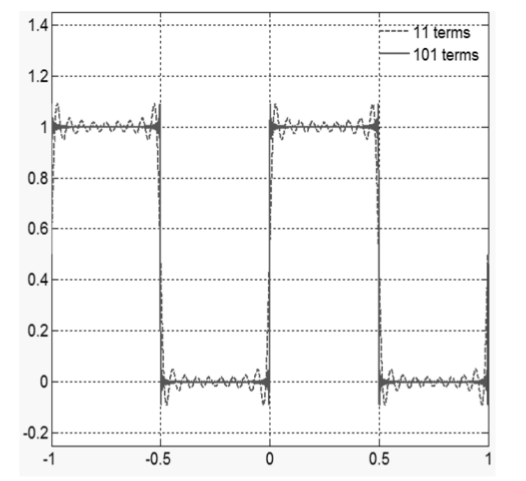
\includegraphics[width=.6\textwidth]{./images/fourier.png}}
  \centering
  \caption{Fourier series representation for a square wave with 11 and 101 terms as in Eq. \ref{Fourier6} \cite{FourierBook}.}
  \label{fPaper1}
\end{figure}

The under and overshoot get closer to the discontinuity with increas-
ing number of terms such that the area under them tends to zero. In
other words they do not contribute to the energy in the function.
This type of convergence is termed as uniform convergence or “al-
most everywhere” convergence (convergence everywhere except on
sets of measure zero). Figure 2.2 shows a region near the disconti-
nuity of the square wave in Fig. 2.1 to illustrate the behaviour of the
Fourier series representation as the number of terms increases. We
may express the uniform convergence property as follows:
\begin{flalign}
	\label{Fourier8}
	\lim _{N\rightarrow \infty} \parallel g(x)-\frac{1}{2}-\sum _{n=0}^{N}\frac{1}{(2n+1)}sin\left [ \frac{2\pi (2n+1)x}{T} \right ] \parallel ^{2}=0.
\end{flalign}
The notation above for the L2-norm square is to be understood as:
\begin{flalign}
	\label{Fourier9}
	\parallel g(x)\parallel^{2} =\int _{-\infty}^{\infty}dx\text{ }\mid g(x)\mid^{2}.
\end{flalign}
As stated above the uniform convergence implies that g(x) and its
approximation need not coincide at every point. The overshoot near
the point of discontinuity can be estimated using a Fourier series
with finite number of terms. Let us consider the partial sum:
\begin{flalign}
	\label{Fourier10}
	S_N(x)=\sum _{n=0}^{N}\frac{1}{(2n+1)}sin\left (\frac{2\pi (2n+1)x}{T} \right ).
\end{flalign}
Taking a derivative of this partial sum with respect to x gives:
\begin{flalign}
	\label{Fourier11}
	S'_N(x)=\frac{2\pi }{T}\sum _{n=0}^{N}cos\left ( \frac{2\pi (2n+1)x}{T} \right ).
\end{flalign}
Summing of this series requires a trick. We note that the consecu-
tive terms of the series have arguments inside the cos(...) function

\begin{flalign*}
	S'_N(x)sin\left ( \frac{4\pi}{T} \right )=\frac{\pi }{T}\left \{
	sin\frac{2\pi (2N+3)x}{T}+sin\frac{2\pi (2N+1)x}{T}
	 \right \}
\end{flalign*}
\begin{flalign}
	\label{Fourier12}
	=\frac{2\pi }{T}sin\left ( \frac{2\pi (2N+2)x}{T} \right )cos\frac{2\pi x}{T}
\end{flalign}
The derivative can thus be expressed as:
\begin{flalign}
	\label{Fourier13}
	S'_N(x)=\left ( \frac{\pi }{T} \right )\left ( \frac{
	sin\left ( \frac{4\pi (N+1)x}{T} \right )
	}{
	sin \left ( \frac{2\pi x}{T} \right )
	} \right ).
\end{flalign}
As we move from the discontinuity at x = 0 to right on the x-axis,
the first maximum of the partial sum in Eq. (2.16) occurs at the place
where the derivative is zero for the first time (one may verify this
by going to second derivatives and checking the sign) at the point:
\begin{flalign*}
	S_N(x_0)=\sum _{n=0}^{N}\frac{1}{(2n+1)}sin\left ( \frac{
	\pi (2n+1)
	}{
	2(N+1)
	} \right )	
\end{flalign*}
\begin{flalign}
	\label{Fourier14}
	=\frac{\pi }{2}\sum _{n=0}^{N}\frac{1}{(N+1)}sinc\left ( \frac{n+\frac{1}{2}}{(N+1)} \right )
\end{flalign}
where we have used the definition:
\begin{flalign}
	\label{Fourier15}
	sinc(x)=\frac{sin\pi x}{\pi x}.
\end{flalign}
For large N the partial sum at x = x 0 above is an approximation
of the integral of the sinc function on interval (0, 1). We therefore
write:
\begin{flalign}
	\label{Fourier16}
	S_N\left ( \frac{T}{4(N+1)} \right )
	\approx \frac{\pi }{2}
	\int _0^{1}dx\text{ }sinc(x).
\end{flalign}
\begin{flalign}
	\label{Fourier17}
	g\left ( \frac{T}{4(N+1)} \right )
	\approx 
	\frac{1}{2}+\int _0^{1}dx\text{ }sinc(x)
	\approx 
	1.0895.
\end{flalign}
The graph of function thus shoots above the square wave by approx-
imately 9